% Public source snapshot: implementation blocks whose provenance has not been
% cleared have been omitted. See sources/README.md for the project's stricter
% independent-provenance and licensing boundary.
\documentclass{article}
\usepackage{graphicx}
\usepackage{amsmath}
\usepackage{amssymb}
\usepackage{listings}
\usepackage[margin=1in]{geometry}
\usepackage{xcolor}
\usepackage{tikz}
\usetikzlibrary{shapes, arrows, positioning, calc}
\usepackage{tcolorbox}

% Define colors for syntax highlighting
\definecolor{codegreen}{rgb}{0,0.6,0}
\definecolor{codegray}{rgb}{0.5,0.5,0.5}
\definecolor{codepurple}{rgb}{0.58,0,0.82}
\definecolor{backcolour}{rgb}{0.95,0.95,0.92}

% Python style for highlighting
\lstdefinestyle{pythonstyle}{
    backgroundcolor=\color{backcolour},
    commentstyle=\color{codegreen},
    keywordstyle=\color{magenta},
    numberstyle=\tiny\color{codegray},
    stringstyle=\color{codepurple},
    basicstyle=\ttfamily\footnotesize,
    breakatwhitespace=false,
    breaklines=true,
    captionpos=b,
    keepspaces=true,
    numbers=left,
    numbersep=5pt,
    showspaces=false,
    showstringspaces=false,
    showtabs=false,
    tabsize=2
}
\lstset{style=pythonstyle}

\title{Lecture: Stabilizing the Information Highway\\
Normalization in Transformers}
\author{Deep Learning Class}
\date{\today}

\begin{document}
\maketitle

\section{Residual Connections}

In a deep network with $L$ layers, gradients are the product of $L$ Jacobian matrices. Even small deviations from perfect conditioning ($\sigma_{\max} \approx 1$) compound exponentially, leading to either explosion or vanishing.
So we need a mechanism to keep activations at a \textbf{predictable, stable scale} throughout the network.

Before we solve the stability problem, we need to understand the architectural feature that makes deep Transformers possible in the first place: \textbf{residual connections}.

Each Transformer layer computes:
\begin{align}
\text{After attention:} \quad &X' = X + \text{Attention}(X) \\
\text{After FFN:} \quad &X'' = X' + \text{FFN}(X')
\end{align}

The key pattern: $X_{\text{out}} = X_{\text{in}} + \text{Block}(X_{\text{in}})$

\begin{center}
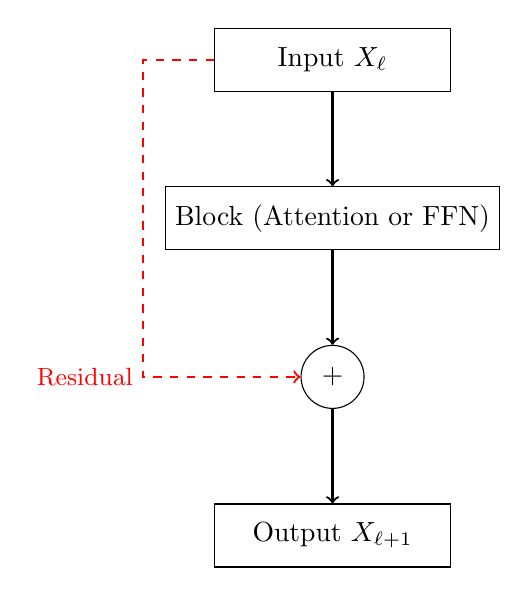
\begin{tikzpicture}[scale=0.9, node distance=1.2cm]
\node[draw, rectangle, minimum width=3cm, minimum height=0.8cm] (input) {Input $X_\ell$};

\node[draw, rectangle, minimum width=3cm, minimum height=0.8cm, below=of input] (block) {Block (Attention or FFN)};

\node[draw, circle, minimum size=0.8cm, below=of block] (add) {$+$};

\node[draw, rectangle, minimum width=3cm, minimum height=0.8cm, below=of add] (output) {Output $X_{\ell+1}$};

\draw[->, thick] (input) -- (block);
\draw[->, thick] (block) -- (add);
\draw[->, thick, dashed, red] (input.west) -- ++(-1,0) |- (add.west) node[midway, left, font=\small] {Residual};
\draw[->, thick] (add) -- (output);
\end{tikzpicture}
\end{center}

\section{The Problem Residuals Create: Scale Drift}

Residual connections enable depth, but they introduce a critical problem.

\subsection{Variance Accumulation in Residual Paths}

Consider what happens as we add multiple blocks:
\begin{align}
X_1 &= X_0 + \text{Block}_1(X_0) \\
X_2 &= X_1 + \text{Block}_2(X_1) = X_0 + \text{Block}_1(X_0) + \text{Block}_2(X_1) \\
X_3 &= X_2 + \text{Block}_3(X_2) = X_0 + \sum_{i=1}^3 \text{Block}_i(\cdots)
\end{align}

Each block output has some variance $\sigma^2_{\text{block}}$. When we add these outputs to the residual stream, the variances add:
\[
\text{Var}(X_\ell) \approx \text{Var}(X_0) + \ell \cdot \sigma^2_{\text{block}}
\]

\textbf{The consequence:} The magnitude (scale) of activations grows as $\sqrt{\ell}$ with depth!

\begin{center}
\begin{tikzpicture}[scale=0.9]
\draw[->] (0,0) -- (10,0) node[right] {Layer depth $\ell$};
\draw[->] (0,0) -- (0,5) node[above] {Activation magnitude};

\draw[thick, blue, domain=0:9, samples=50] plot (\x, {0.5 + 0.3*sqrt(\x)});

\node[blue, align=center] at (7, 3.5) {Scale grows\\as $\sqrt{\ell}$};

\draw[thick, red, dashed] (0,2) -- (9,2) node[right] {Target range};
\end{tikzpicture}
\end{center}

\subsection{Scale Drift Leads to Exploding Gradients}

For any random variable $X$,  $Var(aX+b)=a^2 Var(X)$. The shift $b$ changes the mean, only the scale $\alpha$ changes the variance.

As the scale of $X_\ell$ grows, the gradients $\frac{\partial \mathcal{L}}{\partial X_\ell}$ also grow. Consider:
\begin{itemize}
\item In attention: $\text{score}(i,j) = \frac{q_i^T k_j}{\sqrt{d_k}}$. If $q$ and $k$ have doubled in magnitude, the scores quadruple before scaling!
\item In FFN: $y = W_2 \sigma(W_1 x)$. If $x$ is $2\times$ larger, gradients through $W_1$ are $2\times$ larger.
\end{itemize}

\begin{tcolorbox}[colback=red!5!white, colframe=red!75!black, title=The Scale Drift Problem]
\textbf{The mechanism:} Each residual addition injects variance into the stream.

\textbf{The accumulation:} Over $L$ layers, the scale of activations grows as $O(\sqrt{L})$.

\textbf{The consequence:} Large activations lead to large gradients. Training becomes unstable, diverges, or requires extremely careful hyperparameter tuning.

\textbf{What we need:} A mechanism to \textit{control} the scale of the residual stream, preventing unbounded growth while preserving the information highway.
\end{tcolorbox}

\section{From Batch Norm to Layer Norm}

Normalization transforms activations to have predictable statistics (typically zero mean and unit variance). You already know \textbf{Batch Normalization (BatchNorm)} from CNNs. Let us use it to understand Layer Normalization.

\subsection{Batch Normalization: A Quick Recap}

At each layer, you have $B$ samples in a batch, each producing a $d$-dimensional activation vector. BatchNorm normalizes \textit{across the batch dimension}:

\textbf{For the $i$-th dimension:}
\begin{align}
\mu_i &= \frac{1}{B} \sum_{b=1}^B a_b^{(i)} \quad \text{(mean over batch)} \\
\sigma_i^2 &= \frac{1}{B} \sum_{b=1}^B (a_b^{(i)} - \mu_i)^2 \quad \text{(variance over batch)} \\
\hat{a}_b^{(i)} &= \frac{a_b^{(i)} - \mu_i}{\sqrt{\sigma_i^2 + \epsilon}} \gamma_i + \beta_i
\end{align}

Here, $\mu$ and $\sigma$ are $d$-dimensional vectors (one value per feature dimension), computed by averaging over the $B$ samples.

\textbf{Key point:} BatchNorm creates dependencies between samples in a batch. All samples contribute to computing $\mu$ and $\sigma$.

\subsection{Why Batch Norm Fails for Transformers}

BatchNorm is problematic for sequence models:

\begin{enumerate}
\item \textbf{Variable sequence lengths:} Different sequences have different lengths. Normalizing across sequences with different lengths is awkward.

\item \textbf{Small effective batch sizes:} Long sequences consume lots of memory, forcing small batch sizes. Statistics from small batches are noisy and unreliable.

\item \textbf{Train-test mismatch:} BatchNorm uses batch statistics during training but running averages during inference, causing potential discrepancies.
\end{enumerate}

\textbf{We need something that works independently for each sample.}

\subsection{Layer Normalization: Flip the Averaging Axis}

\textbf{Layer Normalization (LayerNorm)} is like BatchNorm, but normalizes \textit{across the feature dimension} instead of across the batch:

\textbf{For a single sample with activation vector $a \in \mathbb{R}^d$:}
\begin{align}
\mu &= \frac{1}{d} \sum_{j=1}^d a_j \quad \text{(mean over dimensions)} \\
\sigma^2 &= \frac{1}{d} \sum_{j=1}^d (a_j - \mu)^2 \quad \text{(variance over dimensions)} \\
\text{LN}(a) &= \frac{a - \mu}{\sqrt{\sigma^2 + \epsilon}} \odot \gamma + \beta
\end{align}

Here, $\mu$ and $\sigma$ are \textit{scalars} (single numbers) computed by averaging over the $d$ feature dimensions of one sample.

\begin{center}
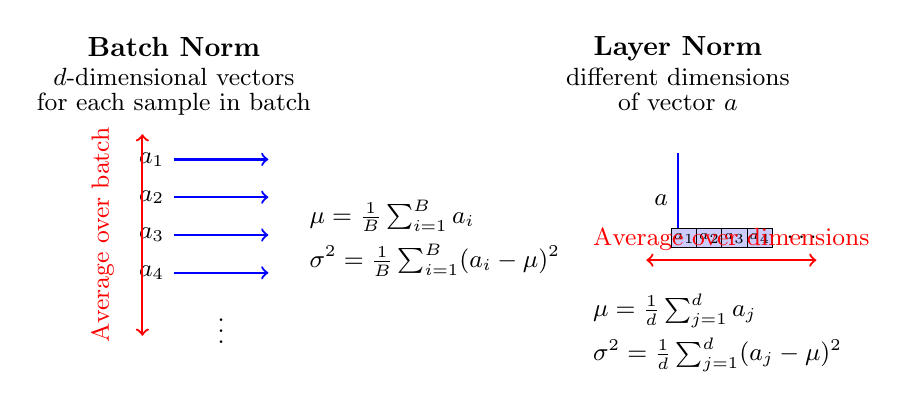
\begin{tikzpicture}[scale=0.8]
% Batch Norm
\begin{scope}
\node[anchor=north] at (0, 5.5) {\textbf{Batch Norm}};
\node[anchor=north, font=\small] at (0, 5) {$d$-dimensional vectors};
\node[anchor=north, font=\small] at (0, 4.6) {for each sample in batch};

% Draw vectors
\foreach \i in {1,2,3,4} {
    \draw[thick, blue, ->] (0, 4-\i*0.6) -- (1.5, 4-\i*0.6);
    \node[left, font=\small] at (0, 4-\i*0.6) {$a_{\i}$};
}
\node[font=\small] at (0.75, 0.8) {$\vdots$};

% Statistics
\node[anchor=west, font=\small, align=left] at (2, 2.5) {$\mu = \frac{1}{B} \sum_{i=1}^B a_i$};
\node[anchor=west, font=\small, align=left] at (2, 1.8) {$\sigma^2 = \frac{1}{B} \sum_{i=1}^B (a_i - \mu)^2$};

\draw[red, thick, <->] (-0.5, 3.8) -- (-0.5, 0.6);
\node[red, font=\small, rotate=90, anchor=south] at (-0.8, 2.2) {Average over batch};
\end{scope}

% Layer Norm
\begin{scope}[xshift=8cm]
\node[anchor=north] at (0, 5.5) {\textbf{Layer Norm}};
\node[anchor=north, font=\small] at (0, 5) {different dimensions};
\node[anchor=north, font=\small] at (0, 4.6) {of vector $a$};

% Draw single vector with dimensions
\draw[thick, blue, ->] (0, 3.5) -- (0, 2);
\node[left, font=\small] at (0, 2.75) {$a$};

% Show dimensions
\foreach \j in {1,2,3,4} {
    \draw[fill=blue!20] (-0.5+\j*0.4, 2) rectangle (-0.1+\j*0.4, 2.3);
    \node[font=\tiny] at (-0.3+\j*0.4, 2.15) {$a_{\j}$};
}
\node[font=\small] at (2, 2.15) {$\cdots$};

% Statistics
\node[anchor=west, font=\small, align=left] at (-1.5, 1) {$\mu = \frac{1}{d} \sum_{j=1}^d a_j$};
\node[anchor=west, font=\small, align=left] at (-1.5, 0.3) {$\sigma^2 = \frac{1}{d} \sum_{j=1}^d (a_j - \mu)^2$};

\draw[red, thick, <->] (-0.5, 1.8) -- (2.2, 1.8);
\node[red, font=\small, anchor=south] at (0.85, 1.8) {Average over dimensions};
\end{scope}
\end{tikzpicture}
\end{center}

\subsection{The Critical Difference}

\begin{tabular}{l|l|l}
& \textbf{Batch Norm} & \textbf{Layer Norm} \\
\hline
Normalize over & $B$ samples & $d$ dimensions \\
$\mu, \sigma$ shape & $d$-dimensional vectors & Scalars (per sample) \\
Dependencies & Across batch & Within sample \\
Batch size sensitivity & Yes (fails for small batches) & No \\
Variable lengths & Problematic & Natural \\
\end{tabular}

\textbf{Layer Norm is like a traditional layer:} It processes each sample independently, making it perfect for sequence models with variable lengths and small batches.

\subsection{Learnable Parameters: Why $\gamma$ and $\beta$?}

Just like BatchNorm, LayerNorm includes learnable affine parameters $\gamma, \beta \in \mathbb{R}^d$:
\[
y = \gamma \odot \frac{a - \mu}{\sqrt{\sigma^2 + \epsilon}} + \beta
\]

\textbf{Why?} Pure normalization fixes mean to 0 and variance to 1, which constrains expressivity:
\begin{itemize}
\item Cannot represent identity: If $f(x) = x$ is optimal, pure normalization cannot represent it
\item Cannot shift operating points: Nonlinearities like GeLU work best in specific ranges; $\gamma$ and $\beta$ let the model learn these optimal regimes
\item Preserves capacity: Allows the normalized representation to realize arbitrary per-feature rescalings and shifts
\end{itemize}

Normalization tames optimization by fixing scale. Learnable parameters restore the degrees of freedom so the model can still represent rich functions.

\section{Architectural Placement: Post-LN vs Pre-LN}

Where we place LayerNorm within the Transformer block profoundly affects training dynamics.

\subsection{Post-Layer Normalization (Post-LN)}

The original Transformer (Vaswani et al., 2017) placed normalization \textit{after} the residual addition:

\begin{center}
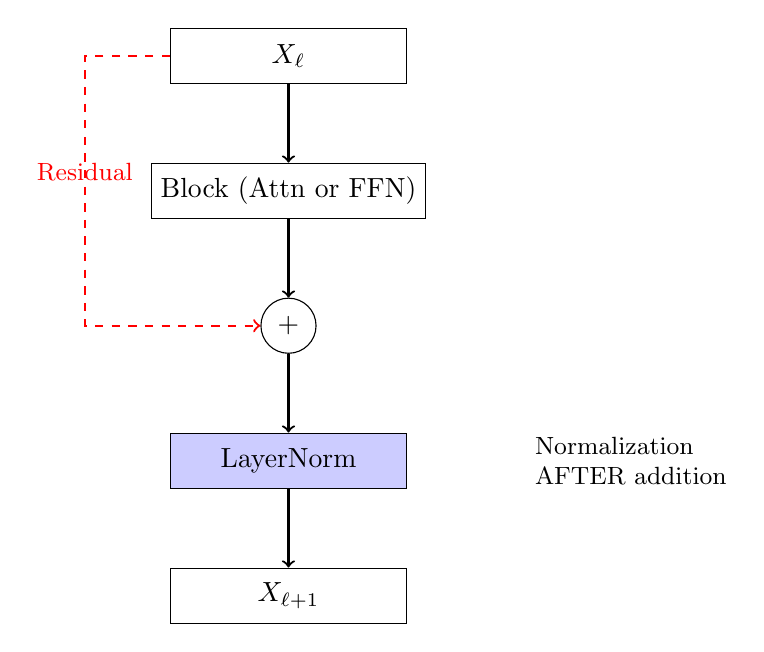
\begin{tikzpicture}[scale=0.9, node distance=1cm]
\node[draw, rectangle, minimum width=3cm, minimum height=0.7cm] (input) {$X_\ell$};

\node[draw, rectangle, minimum width=3cm, minimum height=0.7cm, below=of input] (block) {Block (Attn or FFN)};

\node[draw, circle, minimum size=0.7cm, below=of block] (add) {$+$};

\node[draw, rectangle, minimum width=3cm, minimum height=0.7cm, fill=blue!20, below=of add] (ln) {LayerNorm};

\node[draw, rectangle, minimum width=3cm, minimum height=0.7cm, below=of ln] (output) {$X_{\ell+1}$};

\draw[->, thick] (input) -- (block);
\draw[->, thick] (block) -- (add);
\draw[->, thick, dashed, red] (input.west) -- ++(-1.2,0) |- (add.west) node[near start, above, font=\small] {Residual};
\draw[->, thick] (add) -- (ln);
\draw[->, thick] (ln) -- (output);

\node[right=1.5cm of ln, align=left, font=\small] {Normalization\\AFTER addition};
\end{tikzpicture}
\end{center}

\textbf{Equation:}
\[
X_{\ell+1} = \text{LN}(X_\ell + \text{Block}(X_\ell))
\]

\subsection{The Problem with Post-LN}

In Post-LN, the residual stream passes through the normalization layer. During backpropagation, gradients must flow backward through LayerNorm's complex Jacobian:
\[
\frac{\partial \text{LN}(x)}{\partial x} = \frac{\gamma}{\sigma} \left(I - \frac{1}{d}\mathbf{1}\mathbf{1}^T - \frac{(x-\mu)(x-\mu)^T}{\sigma^2}\right)
\]

Early in training with random initialization, activations have large variance, making the Jacobian's behavior unpredictable. This causes training instability.

\textbf{The workaround:} Post-LN requires \textbf{learning rate warmup} starting from tiny learning rates (e.g., $10^{-7}$) and gradually increasing over thousands of steps. This is tedious to tune and slows early training.

\subsection{Pre-Layer Normalization (Pre-LN)}

A key architectural innovation: move normalization to the \textit{beginning} of each block:

\begin{center}
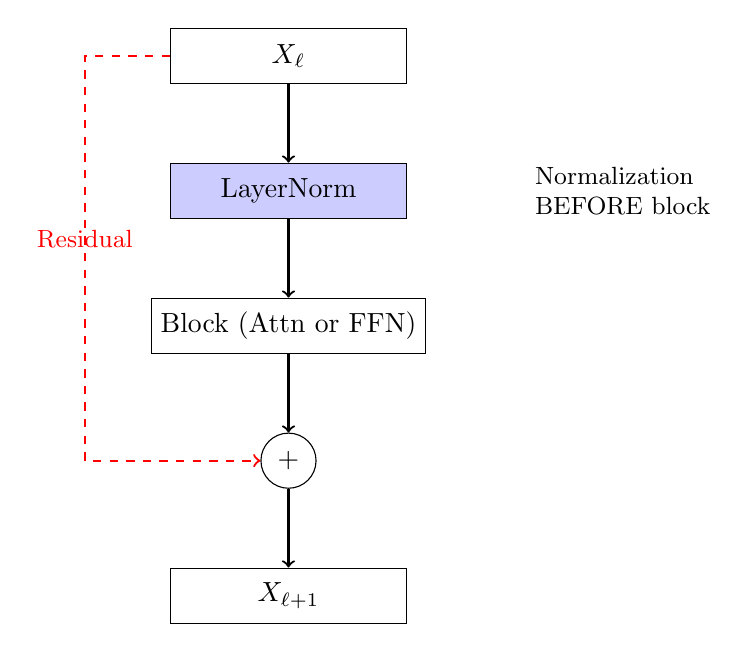
\begin{tikzpicture}[scale=0.9, node distance=1cm]
\node[draw, rectangle, minimum width=3cm, minimum height=0.7cm] (input) {$X_\ell$};

\node[draw, rectangle, minimum width=3cm, minimum height=0.7cm, fill=blue!20, below=of input] (ln) {LayerNorm};

\node[draw, rectangle, minimum width=3cm, minimum height=0.7cm, below=of ln] (block) {Block (Attn or FFN)};

\node[draw, circle, minimum size=0.7cm, below=of block] (add) {$+$};

\node[draw, rectangle, minimum width=3cm, minimum height=0.7cm, below=of add] (output) {$X_{\ell+1}$};

\draw[->, thick] (input) -- (ln);
\draw[->, thick] (ln) -- (block);
\draw[->, thick] (block) -- (add);
\draw[->, thick, dashed, red] (input.west) -- ++(-1.2,0) |- (add.west) node[near start, above, font=\small] {Residual};
\draw[->, thick] (add) -- (output);

\node[right=1.5cm of ln, align=left, font=\small] {Normalization\\BEFORE block};
\end{tikzpicture}
\end{center}

\textbf{Equation:}
\[
X_{\ell+1} = X_\ell + \text{Block}(\text{LN}(X_\ell))
\]

\subsection{Why Pre-LN is More Stable}

The key difference: the residual stream now provides a \textbf{clean gradient path}.

\textbf{Gradient flow in Pre-LN:}
\[
\frac{\partial \mathcal{L}}{\partial X_\ell} = \frac{\partial \mathcal{L}}{\partial X_{\ell+1}} \left(I + \frac{\partial \text{Block}}{\partial \text{LN}(X_\ell)} \frac{\partial \text{LN}(X_\ell)}{\partial X_\ell}\right)
\]

The identity term $I$ allows gradients to flow backward \textit{without} passing through the LayerNorm Jacobian!

\begin{center}
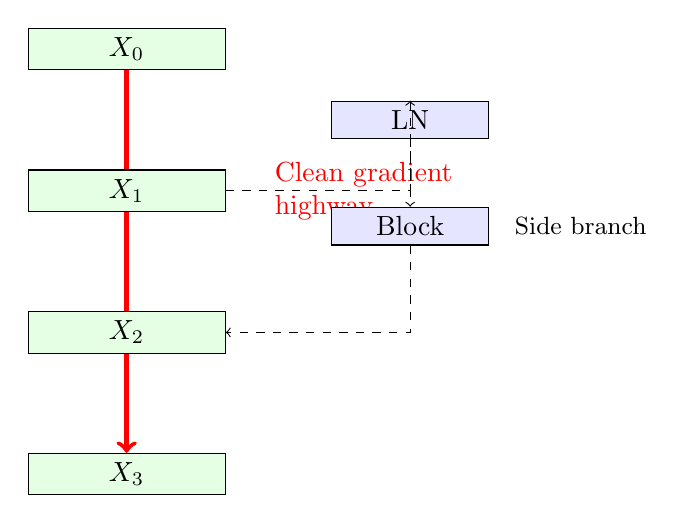
\begin{tikzpicture}[scale=0.9]
\node[draw, rectangle, minimum width=2.5cm, fill=green!10] (x3) at (0,0) {$X_3$};
\node[draw, rectangle, minimum width=2.5cm, fill=green!10] (x2) at (0,2) {$X_2$};
\node[draw, rectangle, minimum width=2.5cm, fill=green!10] (x1) at (0,4) {$X_1$};
\node[draw, rectangle, minimum width=2.5cm, fill=green!10] (x0) at (0,6) {$X_0$};

\draw[->, ultra thick, red] (x0) -- (x1) -- (x2) -- (x3);
\node[right=0.5cm of x1, align=left, red] {Clean gradient\\highway};

\node[draw, rectangle, minimum width=2cm, fill=blue!10] (ln1) at (4,5) {LN};
\node[draw, rectangle, minimum width=2cm, fill=blue!10] (blk1) at (4,3.5) {Block};

\draw[->, dashed] (x1.east) -| (ln1.north);
\draw[->, dashed] (ln1) -- (blk1);
\draw[->, dashed] (blk1.south) |- (x2.east);

\node[right=0.2cm of blk1, font=\small] {Side branch};
\end{tikzpicture}
\end{center}

\textbf{Benefits of Pre-LN:}
\begin{enumerate}
\item Stable gradients via identity path that bypasses normalization
\item No warmup needed---training can start with normal learning rates
\item Can train 100+ layer Transformers reliably
\item Better initialization robustness
\end{enumerate}

\begin{tcolorbox}[colback=green!5!white, colframe=green!50!black, title=Pre-LN: The Modern Standard]
Pre-Layer Normalization has become the dominant architecture for Transformers because it provides a clean gradient highway via the residual stream, dramatically improving training stability and enabling much deeper models without warmup.

\textbf{Modern practice:} Almost all state-of-the-art Transformers (GPT-3, LLaMA, PaLM, Mistral) use Pre-LN.
\end{tcolorbox}

\section{The Optimization: Root Mean Square Normalization (RMSNorm)}

With Pre-LN established as the standard, researchers began analyzing LayerNorm more carefully. A key question emerged: \textit{do we need both centering and scaling?}

\subsection{The Key Empirical Insight}

Through extensive experiments on deep Pre-LN Transformers, researchers observed:

\begin{tcolorbox}[colback=blue!5!white, colframe=blue!50!black, title=The Centering vs Scaling Question]
\textbf{Observation:} In Pre-LN Transformers, the \textbf{scaling} operation (controlling magnitude) is critical for stable gradients.

\textbf{Observation:} The \textbf{centering} operation (subtracting mean) contributes much less to training stability.

\textbf{Implication:} We can simplify LayerNorm by removing centering!
\end{tcolorbox}

\subsection{Introducing RMSNorm}

\textbf{Root Mean Square Normalization (RMSNorm)} keeps only the scaling operation:

\[
\text{RMS}(x) = \sqrt{\frac{1}{d}\sum_{i=1}^d x_i^2 + \epsilon}
\]

\[
\text{RMSNorm}(x) = \frac{x}{\text{RMS}(x)} \odot \gamma
\]

\textbf{Compare to LayerNorm:}
\begin{align}
\text{LayerNorm}(x) &= \frac{x - \mu}{\sqrt{\sigma^2 + \epsilon}} \odot \gamma + \beta \\
\text{RMSNorm}(x) &= \frac{x}{\text{RMS}(x)} \odot \gamma
\end{align}

\textbf{Key differences:}
\begin{itemize}
\item \textbf{No mean subtraction:} RMSNorm does not center the data
\item \textbf{No bias parameter:} Only $\gamma$ (gain), no $\beta$ (shift)
\item \textbf{Direct magnitude normalization:} Divides by RMS instead of standard deviation after centering
\end{itemize}

RMS measures magnitude directly from the origin, proportional to the $\ell_2$ norm: $\text{RMS}(x) = \frac{\|x\|_2}{\sqrt{d}}$. RMSNorm projects each vector onto the unit sphere (after accounting for dimension), preserving direction while fixing scale.

\section{Why RMSNorm is Superior in Modern LLMs}

RMSNorm has rapidly become the standard in modern large language models (LLaMA, T5, Mistral, Gemma, etc.).

\subsection{Advantage 1: Numerical Stability in Low Precision}

Modern training relies on low-precision arithmetic (fp16, bf16). LayerNorm computes $x - \mu$, which causes \textbf{catastrophic cancellation} when $x$ and $\mu$ are close:

\textbf{Example in fp16:} If $x = 1.2345678$ stored as $1.234$ and $\mu = 1.2345123$ stored as $1.234$, then $x - \mu$ should be $0.0000555$ but computes as $0.000$!

RMSNorm only computes $\sum x_i^2$, square root, and division---all numerically stable operations with no subtraction of close numbers.

\subsection{Advantage 2: Computational Efficiency}

\textbf{Operation count for $d$-dimensional vector:}
\begin{itemize}
\item LayerNorm: $\sim 5d$ operations (compute mean, variance, normalize, apply $\gamma, \beta$)
\item RMSNorm: $\sim 3d$ operations (compute $\sum x_i^2$, RMS, normalize and scale)
\end{itemize}

\textbf{Savings:} RMSNorm is roughly 40\% fewer operations!

\textbf{Memory:} RMSNorm has only $d$ parameters ($\gamma$) vs LayerNorm's $2d$ parameters ($\gamma, \beta$).

For LLaMA-65B with 80 normalization layers of dimension 8192: saves 655,360 parameters.

\subsection{Advantage 3: Simpler Gradient Flow}

The Jacobian of RMSNorm is simpler than LayerNorm's:
\[
\frac{\partial \text{RMSNorm}(x)}{\partial x} = \frac{\gamma}{\text{RMS}(x)}\left(I - \frac{xx^T}{\|x\|^2}\right)
\]

The coupling is weaker (no centering term $\frac{1}{d}\mathbf{1}\mathbf{1}^T$ from LayerNorm), leading to smoother optimization.

\subsection{Advantage 4: Preserves Direction, Fixes Scale}

LayerNorm centers then scales, changing the direction of $x$ in feature space. RMSNorm only scales, preserving direction while controlling magnitude. In residual streams, this less invasive transformation often preserves more information.

\begin{tcolorbox}[colback=blue!5!white, colframe=blue!50!black, title=RMSNorm: The Modern Standard]
RMSNorm has become the normalization of choice in modern LLMs because:

\begin{enumerate}
\item \textbf{Numerical stability:} Avoids catastrophic cancellation in low precision
\item \textbf{Efficiency:} 40\% fewer operations, half the parameters
\item \textbf{Simpler gradients:} Weaker feature coupling, smoother optimization
\item \textbf{Sufficient for stability:} In Pre-LN, controlling scale is what matters most
\end{enumerate}

\textbf{Used in:} LLaMA (1, 2, 3), T5, Mistral, Gemma, and most modern open-source LLMs.
\end{tcolorbox}

\section{Practical Considerations and Trade-offs}

\subsection{When to Use LayerNorm vs RMSNorm}

\textbf{Use LayerNorm when:}
\begin{itemize}
\item Working with Post-LN architectures (legacy models)
\item You need guaranteed zero-mean activations for theoretical reasons
\item Working in high precision (fp32) where numerical issues are minimal
\end{itemize}

\textbf{Use RMSNorm when:}
\begin{itemize}
\item Building new Pre-LN Transformers (most modern cases)
\item Training in low precision (fp16, bf16) for efficiency
\item Optimizing for inference speed and memory
\item Building large language models (100M+ parameters)
\end{itemize}

\subsection{Interaction with Other Design Choices}

\textbf{Biases in linear layers:} Many modern architectures drop biases from linear layers when using RMSNorm ($y = Wx$ with no $+b$). LayerNorm's $\beta$ provides a shift, making linear biases partially redundant. RMSNorm has no $\beta$, but the residual stream provides an additive path. Dropping biases saves parameters without hurting performance.

\textbf{Initialization:} LayerNorm: $\gamma = 1, \beta = 0$. RMSNorm: $\gamma = 1$. Some architectures initialize $\gamma$ slightly smaller (e.g., 0.1) to make each block contribute weakly initially.

\textbf{Epsilon ($\epsilon$) tuning:} Typical values: $\epsilon = 10^{-6}$ or $10^{-5}$. In fp16/bf16, may need larger $\epsilon$ to avoid underflow.

\subsection{Does RMSNorm Guarantee Zero Mean?}

\textbf{No.} RMSNorm does not center activations. However, for Pre-LN Transformers trained on language modeling, zero mean does not appear necessary. Models trained with RMSNorm perform as well or better than those with LayerNorm. The residual stream provides an additive path that can shift means as needed.

\section{Implementation}

% LayerNorm, RMSNorm, and Pre/Post-LN implementation examples omitted from the
% public snapshot because their implementation provenance has not been cleared.
% See sources/README.md.

\section{Summary: The Evolution of Normalization in Transformers}

\subsection{The Journey}

\textbf{1. The Problem:} Deep residual networks suffer from scale drift. Variance accumulates as $O(\sqrt{L})$ with depth, leading to exploding/vanishing gradients and unstable training.

\textbf{2. The Initial Solution:} Layer Normalization normalizes across features for each token, centering (zero mean) and scaling (unit variance). Learnable $\gamma, \beta$ restore expressivity.

\textbf{3. The Architectural Insight:} Pre-LN vs Post-LN. Original Transformer used Post-LN (normalize after residual), requiring learning rate warmup and less stability. Pre-LN (normalize before block) provides clean gradient path and is now the modern standard.

\textbf{4. The Optimization:} RMSNorm. In Pre-LN, controlling scale matters more than centering. Remove mean subtraction, keep scaling. Benefits: fewer operations, better numerical stability, fewer parameters. Modern LLMs (LLaMA, Mistral, etc.) use RMSNorm.

\subsection{Key Takeaways}

\begin{enumerate}
\item \textbf{Normalization is essential:} Deep networks need explicit scale control to prevent gradient issues.

\item \textbf{Learnable parameters are crucial:} Pure normalization constrains expressivity. $\gamma$ (and $\beta$) allow the model to recover identity and learn optimal operating points.

\item \textbf{Placement matters:} Pre-LN provides better gradient flow than Post-LN by keeping the residual stream clean.

\item \textbf{Simplification is possible:} In Pre-LN, centering is less critical. RMSNorm achieves comparable or better results with less computation.

\item \textbf{Numerical precision matters:} Low-precision training (fp16/bf16) favors numerically stable operations. RMSNorm avoids catastrophic cancellation.
\end{enumerate}

\begin{tcolorbox}[colback=blue!5!white, colframe=blue!75!black, title=Modern Best Practices]
\textbf{For new Transformer implementations:}
\begin{itemize}
\item Use \textbf{Pre-Layer Normalization} architecture
\item Use \textbf{RMSNorm} for efficiency and stability
\item Initialize $\gamma = 1$
\item Consider dropping biases from linear layers
\item Train in bf16 or fp16 with appropriate $\epsilon$
\end{itemize}

\textbf{These choices reflect years of empirical findings and are used in virtually all modern large language models.}
\end{tcolorbox}

\section{Further Reading}

\subsection{Foundational Papers}

\begin{itemize}
\item Ba, J. L., Kiros, J. R., \& Hinton, G. E. (2016). \textbf{Layer Normalization}. arXiv:1607.06450. \textit{The original LayerNorm paper.}

\item Vaswani, A., et al. (2017). \textbf{Attention Is All You Need}. NeurIPS. \textit{Original Transformer with Post-LN.}

\item Xiong, R., et al. (2020). \textbf{On Layer Normalization in the Transformer Architecture}. ICML. \textit{Analysis of Pre-LN vs Post-LN.}

\item Zhang, B., \& Sennrich, R. (2019). \textbf{Root Mean Square Layer Normalization}. NeurIPS. \textit{Introduction of RMSNorm.}
\end{itemize}

\subsection{Modern Implementations}

\begin{itemize}
\item Touvron, H., et al. (2023). \textbf{LLaMA: Open and Efficient Foundation Language Models}. \textit{Uses Pre-LN + RMSNorm.}

\item Chowdhery, A., et al. (2022). \textbf{PaLM: Scaling Language Modeling with Pathways}. \textit{Pre-LN architecture at 540B scale.}

\item Jiang, A. Q., et al. (2023). \textbf{Mistral 7B}. \textit{Efficient architecture with RMSNorm.}
\end{itemize}

\subsection{Further Topics}

\begin{itemize}
\item \textbf{Other normalization schemes:} GroupNorm, InstanceNorm, their trade-offs with LayerNorm

\item \textbf{Normalization-free architectures:} NFNet, exploring whether normalization is necessary with careful initialization

\item \textbf{Low-precision training:} Mixed precision, gradient scaling, numerical considerations

\item \textbf{Residual scaling:} Techniques like ReZero, Fixup that modify how residuals are added
\end{itemize}

\end{document}
